\documentclass[symmetry,article,accept,pdftex,moreauthors]{Definitions/mdpi} 
%\usepackage{boisik}
%\usepackage[OT1]{fontenc}
%\usepackage[affil-it]{authblk}
%\usepackage{graphicx}
%\usepackage{textcomp}
%\usepackage{multicol}
%\usepackage{natbib}
%\usepackage{geometry}
%\usepackage{amsmath}
%\usepackage{lineno}
%%\usepackage{multirow}
%\usepackage[dvipsnames]{xcolor}
%\usepackage{hyperref}
%\hypersetup{
%    colorlinks,
%    linkcolor={red!50!black},
%    citecolor={blue!50!black},
%    urlcolor={blue!80!black}
%}
%\usepackage{xcolor}
%\usepackage{float}
%\usepackage{wrapfig}
\firstpage{1} 
\makeatletter 
\setcounter{page}{\@firstpage} 
\makeatother
\pubvolume{1}
\issuenum{1}
\articlenumber{0}
\pubyear{2022}
\copyrightyear{2022}
\externaleditor{{Academic Editor}: Pecchinenda Anna} % For journal Automation, please change Academic Editor to "Communicated by"
%mdpi: please add academic editor
\datereceived{23 February 2022} 
\dateaccepted{13 April 2022} 
\datepublished{} 
%\datecorrected{} % Corrected papers include a "Corrected: XXX" date in the original paper.
%\dateretracted{} % Corrected papers include a "Retracted: XXX" date in the original paper.
\hreflink{https://doi.org/} % If needed use \linebreak


%\linenumbers

\Title{Perceptual Similarities Among Wallpaper Group Exemplars}

% MDPI internal command: Title for citation in the left column
\TitleCitation{Perceptual Similarities Among Wallpaper Group Exemplars}

% Author Orchid ID: enter ID or remove command
\newcommand{\orcidauthorA}{0000-0000-0000-000X} % Add \orcidA{} behind the author's name
%\newcommand{\orcidauthorB}{0000-0000-0000-000X} % Add \orcidB{} behind the author's name

% Authors, for the paper (add full first names)
\Author{\hl{Peter J. Kohler} $^{1,2,}$*, Shivam Vedak $^{3}$ and Rick O. Gilmore $^{3}$}
%Please carefully check the accuracy of names and affiliations. Changes will not be possible after proofreading.

%\longauthorlist{yes}

% MDPI internal command: Authors, for metadata in PDF
\AuthorNames{Peter J. Kohler, Shivam Vedak and Rick O. Gilmore}

% MDPI internal command: Authors, for citation in the left column
\AuthorCitation{Kohler, P.J.; Vedak, V.; Gilmore, R.O.}
% If this is a Chicago style journal: Lastname, Firstname, Firstname Lastname, and Firstname Lastname.

% Affiliations / Addresses (Add [1] after \address if there is only one affiliation.)
\address{%
$^{1}$ \quad Department of Psychology, York University, Toronto, ON M3J 1P3, Canada\\
$^{2}$ \quad Centre for Vision Research, York University, Toronto, ON, M3J 1P3, Canada\\
$^{3}$ \quad Department of Psychology, The Pennsylvania State University, State College, PA, 16801, USA; shivam.vedak@gmail.com (S.V.); rog1@psu.edu (R.O.G.)}
%MDPI: please add city and post code

% Contact information of the corresponding author
\corres{Correspondence: pjkohler@yorku.ca}

% Current address and/or shared authorship
%\firstnote{Current address: Affiliation 3} 
%\secondnote{These authors contributed equally to this work.}
% The commands \thirdnote{} till \eighthnote{} are available for further notes

%\simplesumm{} % Simple summary

%\conference{} % An extended version of a conference paper

% Abstract (Do not insert blank lines, i.e. \\) 
\abstract{Symmetries are abundant within the visual environment, and many animals species are sensitive to visual symmetries. Wallpaper groups constitute a class of 17 regular textures that each contain a distinct combination of the four fundamental symmetries, translation, reflection, rotation and glide reflection, and together represent the complete set of possible symmetries in two-dimensional images. Wallpapers are visually compelling and elicit responses in visual brain areas that precisely capture the symmetry content of each group in humans and other primates. Here we ask to what extent \textit{different} exemplars from the \textit{same} wallpaper group are perceptually similar. We used an algorithm to produce a set of well-matched exemplars from 5 of the 17 wallpaper groups and instructed participants to freely sort the exemplars from each group into as many subsets as they wished based on any criteria they saw appropriate. \textit{P1}, the simplest of the 17 groups, was consistently rated more self-similar than any other group, while the other four groups, although varying in symmetry content, were comparable in self-similarity. Our results suggest that except for the most extreme case (\textit{P1}), perceived self-similarity of wallpaper groups is not directly tied to categories of symmetry based on group theory.}

% Keywords
\keyword{wallpaper groups; visual perception; behavioral sorting; self-similarity} 


%\title{\huge Perceptual Similarities Among Wallpaper Group Exemplars}
%\author[1,2]{Peter J. Kohler}
%\author[3]{Shivam Vedak}
%\author[3]{Rick O. Gilmore}
%
%\affil[1]{\small York University, Department of Psychology, Toronto, ON M3J 1P3, Canada}
%\affil[2]{\small Centre for Vision Research, York University, Toronto, ON, M3J 1P3, Canada}
%\affil[3]{\small Department of Psychology, The Pennsylvania State University, Pennsylvania, USA}
%
%\date{}
%
%
%
%
%% about 200 words
%\begin{abstract}Symmetries are abundant within the visual environment, and many animal species are sensitive to visual symmetries. Wallpaper groups constitute a class of 17 regular textures that each contain a distinct combination of the four fundamental symmetries, translation, reflection, rotation and glide reflection, and together represent the complete set of possible symmetries in two-dimensional images. Wallpapers are visually compelling and elicit responses in visual brain areas that precisely capture the symmetry content of each group in humans and other primates. Here we ask to what extent \textit{different} exemplars from the \textit{same} wallpaper group are perceptually similar. We used an algorithm to produce a set of well-matched exemplars from 5 of the 17 wallpaper groups and instructed participants to freely sort the exemplars from each group into as many subsets as they wished, based on any criteria they saw appropriate. \textit{P1}, the simplest of the 17 groups, was consistently rated more self-similar than any other group, while the other four groups, although varying in symmetry content, were comparable in self-similarity. Our results suggest that except for the most extreme case (\textit{P1}), perceived self-similarity of wallpaper groups is not directly tied to categories of symmetry based on group theory.\end{abstract}
%
%\keywords{wallpaper groups, visual perception, behavioral sorting, self-similarity}

\begin{document}
\section{Introduction}
Symmetry exists in an object or pattern if a transformation can be applied that maps the object/pattern onto itself. In the two-dimensional plane, the set of isometries--distance--preserving transformations, see \citep{RN1425}---what can give rise to symmetries are translation, reflection, rotation and glide reflection and their combinations. The \textit{\hl{wallpaper groups(MDPI: is the italic necessary?
)}} are a set of 17 regular textures, where each has a unique combination of isometries that leave the texture unchanged \citep{RN1562,RN1563,RN1425}. Each wallpaper group therefore contains a distinct combination of four symmetry types (see Figure \ref{fig:symmetry_types}). Symmetries have been recognized as important for human visual perception since the late 19th century \citep{mach_1959}.  Wallpaper groups are different from stimuli typically used to probe the role of symmetry in visual perception in two ways: First, they contain combinations of four symmetry types, rather than just reflection (also called mirror symmetry), which have been the focus of most vision research. Second, in wallpaper groups, symmetries are repeated to tile the plane and form textures, instead of being positioned at a single image location, as is usually the case with standard stimuli. These differences, and the important fact that wallpaper groups together form the complete set of symmetries possible in the two-dimensional image plane, make wallpapers an interesting stimulus set for studying the perception of visual symmetries.%MDPI: is the italic necessary?

\begin{figure}[H]

	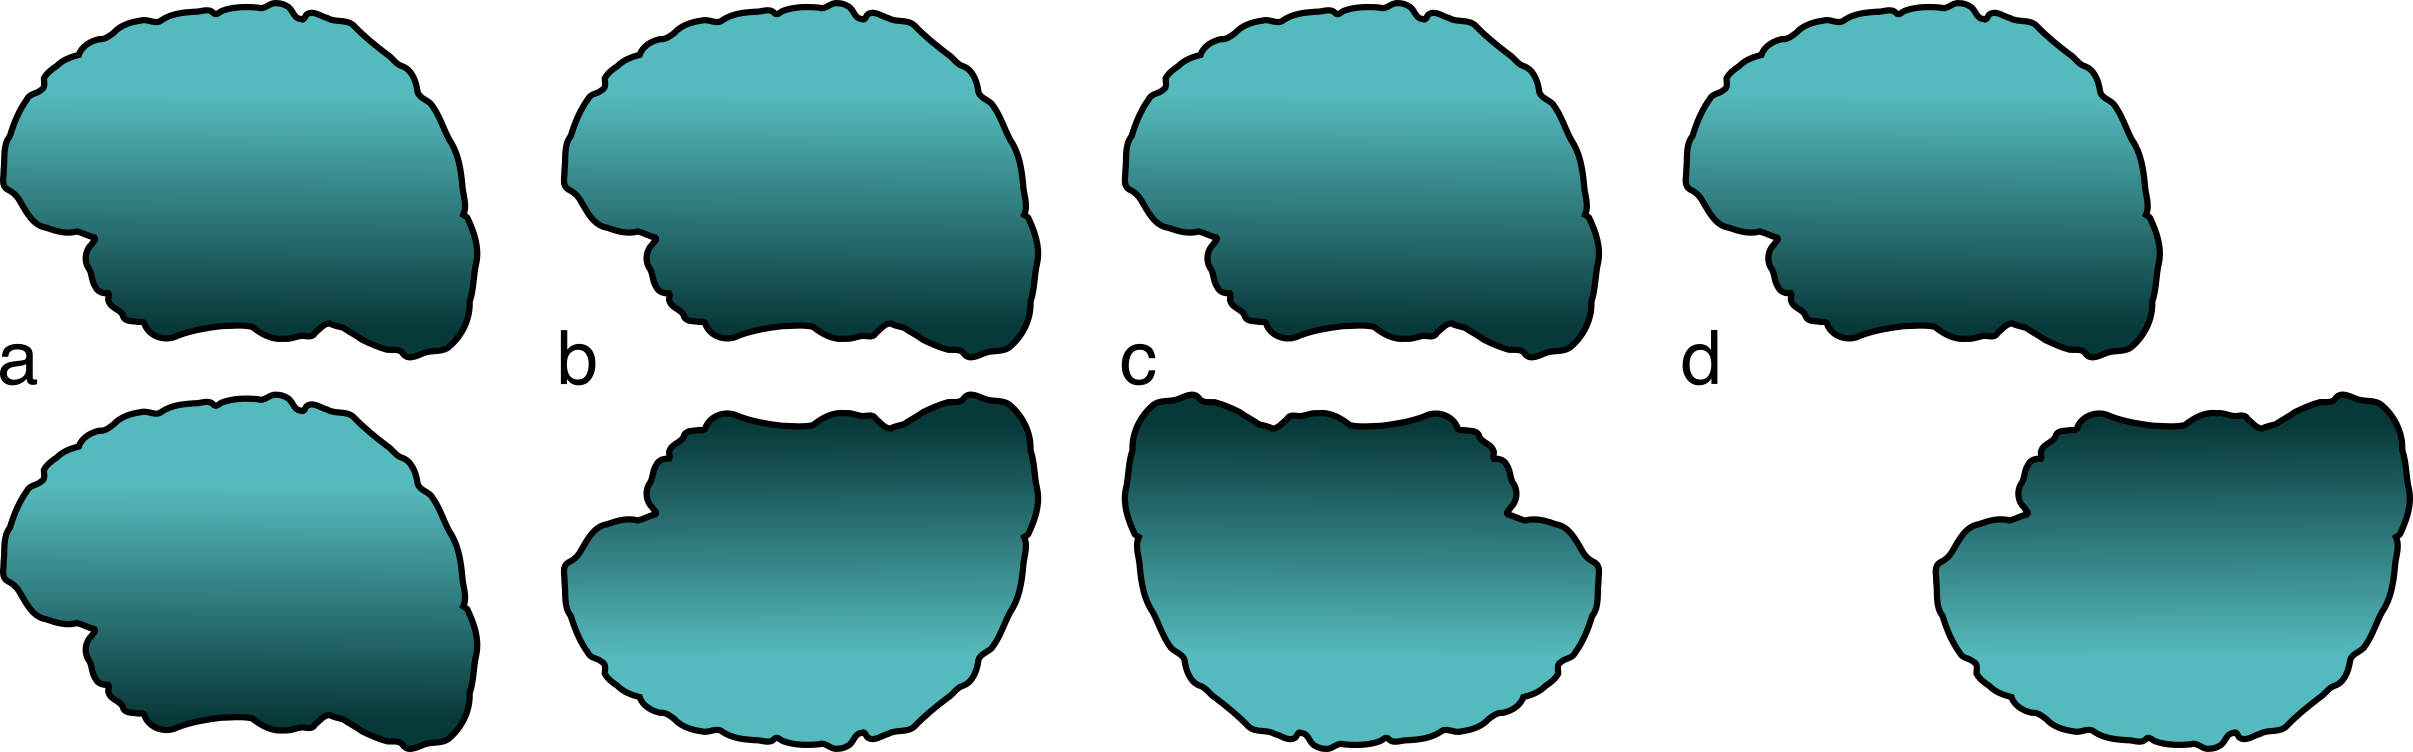
\includegraphics[scale=0.6]{./figures/symmetry_types.png}
	\caption{The four fundamental symmetry types: (\textbf{a}) translation, (\textbf{b}) reflection, (\textbf{c}) rotation (order 2, 180$^{\circ}$) (\textbf{d}) glide reflection--translation followed by reflection over a line parallel to the direction of translation. }
	\label{fig:symmetry_types}
\end{figure}

Brain imaging studies using functional MRI \citep{RN1725} and EEG \citep{RN1959,kohler_clarke_2021} have demonstrated that the human visual system carries detailed and precise representations of the symmetries within the individual wallpaper groups. Specifically, response amplitudes scale approximately linearly with the symmetry content within the wallpaper groups, across all of the possible combinations of reflection, rotation and glide reflection symmetries. Functional MRI evidence from macaque monkeys reveal similar representations in the macaque visual system, and the brain regions responding to symmetry are largely analogous between humans and monkeys, namely the functionally defined regions V3, V4, VO1 and LOC \citep{audurier_symmetry_2021}.


The wallpaper group representations that have been identified using brain imaging are highly complex, but do not appear to be readily available for driving conscious behaviour: Humans have limited intuitive sense of group membership for wallpaper group exemplars, as evidenced by behavioral experiments showing that although naïve observers can distinguish many of the wallpaper groups \citep{RN1253}, they tend to sort exemplars into fewer (4--12) sets than the number of wallpaper groups, often placing exemplars from different groups into the same set \citep{RN172}. Wallpaper groups are nonetheless visually compelling, and anecdotally we have observed that exemplars from a given group can be quite perceptually diverse. This observation inspired the current study. Here, we use behavioral sorting, a common technique to study perceptual categorization \citep{Milton2008-ez,Pothos2011-vi}, to probe the perceptual self-similarity of different exemplars from the same wallpaper group. In previous sorting experiments with wallpaper groups (e.g., \citep{RN172}), observers were shown exemplars from different wallpaper groups, and their ability to correctly sort exemplars from the same group into the same subset was assessed. Our approach was different: We wanted to know the extent to which exemplars from the \textit{same group} would be spontaneously organized into subsets, i.e., the self-similarity of exemplars from a given group. We selected five distinct wallpaper groups: \textit{P1}, \textit{P3M1}, \textit{P31M}, \textit{P6} and \textit{P6M} (see Figure \ref{fig:wpg_structure}). All wallpaper groups consist of a lattice that is repeated to tile the plane. \textit{P1} is the simplest group, and contains no symmetries other than the translation generated by the repeating lattice. \textit{P6} has rotation symmetries of order 6, 3 and 2, but no other symmetries besides translation. \textit{P3M1} and \textit{P31M} both have rotations of order 3, reflections in three distinct directions, and glide reflections in three distinct directions, but differ in terms of how these symmetries are organized in the lattice. \textit{P6M} is the most complex of the groups, it has rotation symmetries of order 6, 3 and 2, reflections in six distinct directions, and glide reflections in six distinct directions. The lattice structure of the five groups is described in detail on the wallpaper group wikipedia page (\url{https://en.wikipedia.org/wiki/Wallpaper_group}, accessed on 14/4/2022). The five groups selected have all been found to have high self-similarity \citep{RN172}, and four of them (\textit{P3M1}, \textit{P31M}, \textit{P6} and \textit{P6M}) share the same lattice shape (see Figure \ref{fig:wpg_structure}). %mdpi: please add date

\begin{figure}[H]

	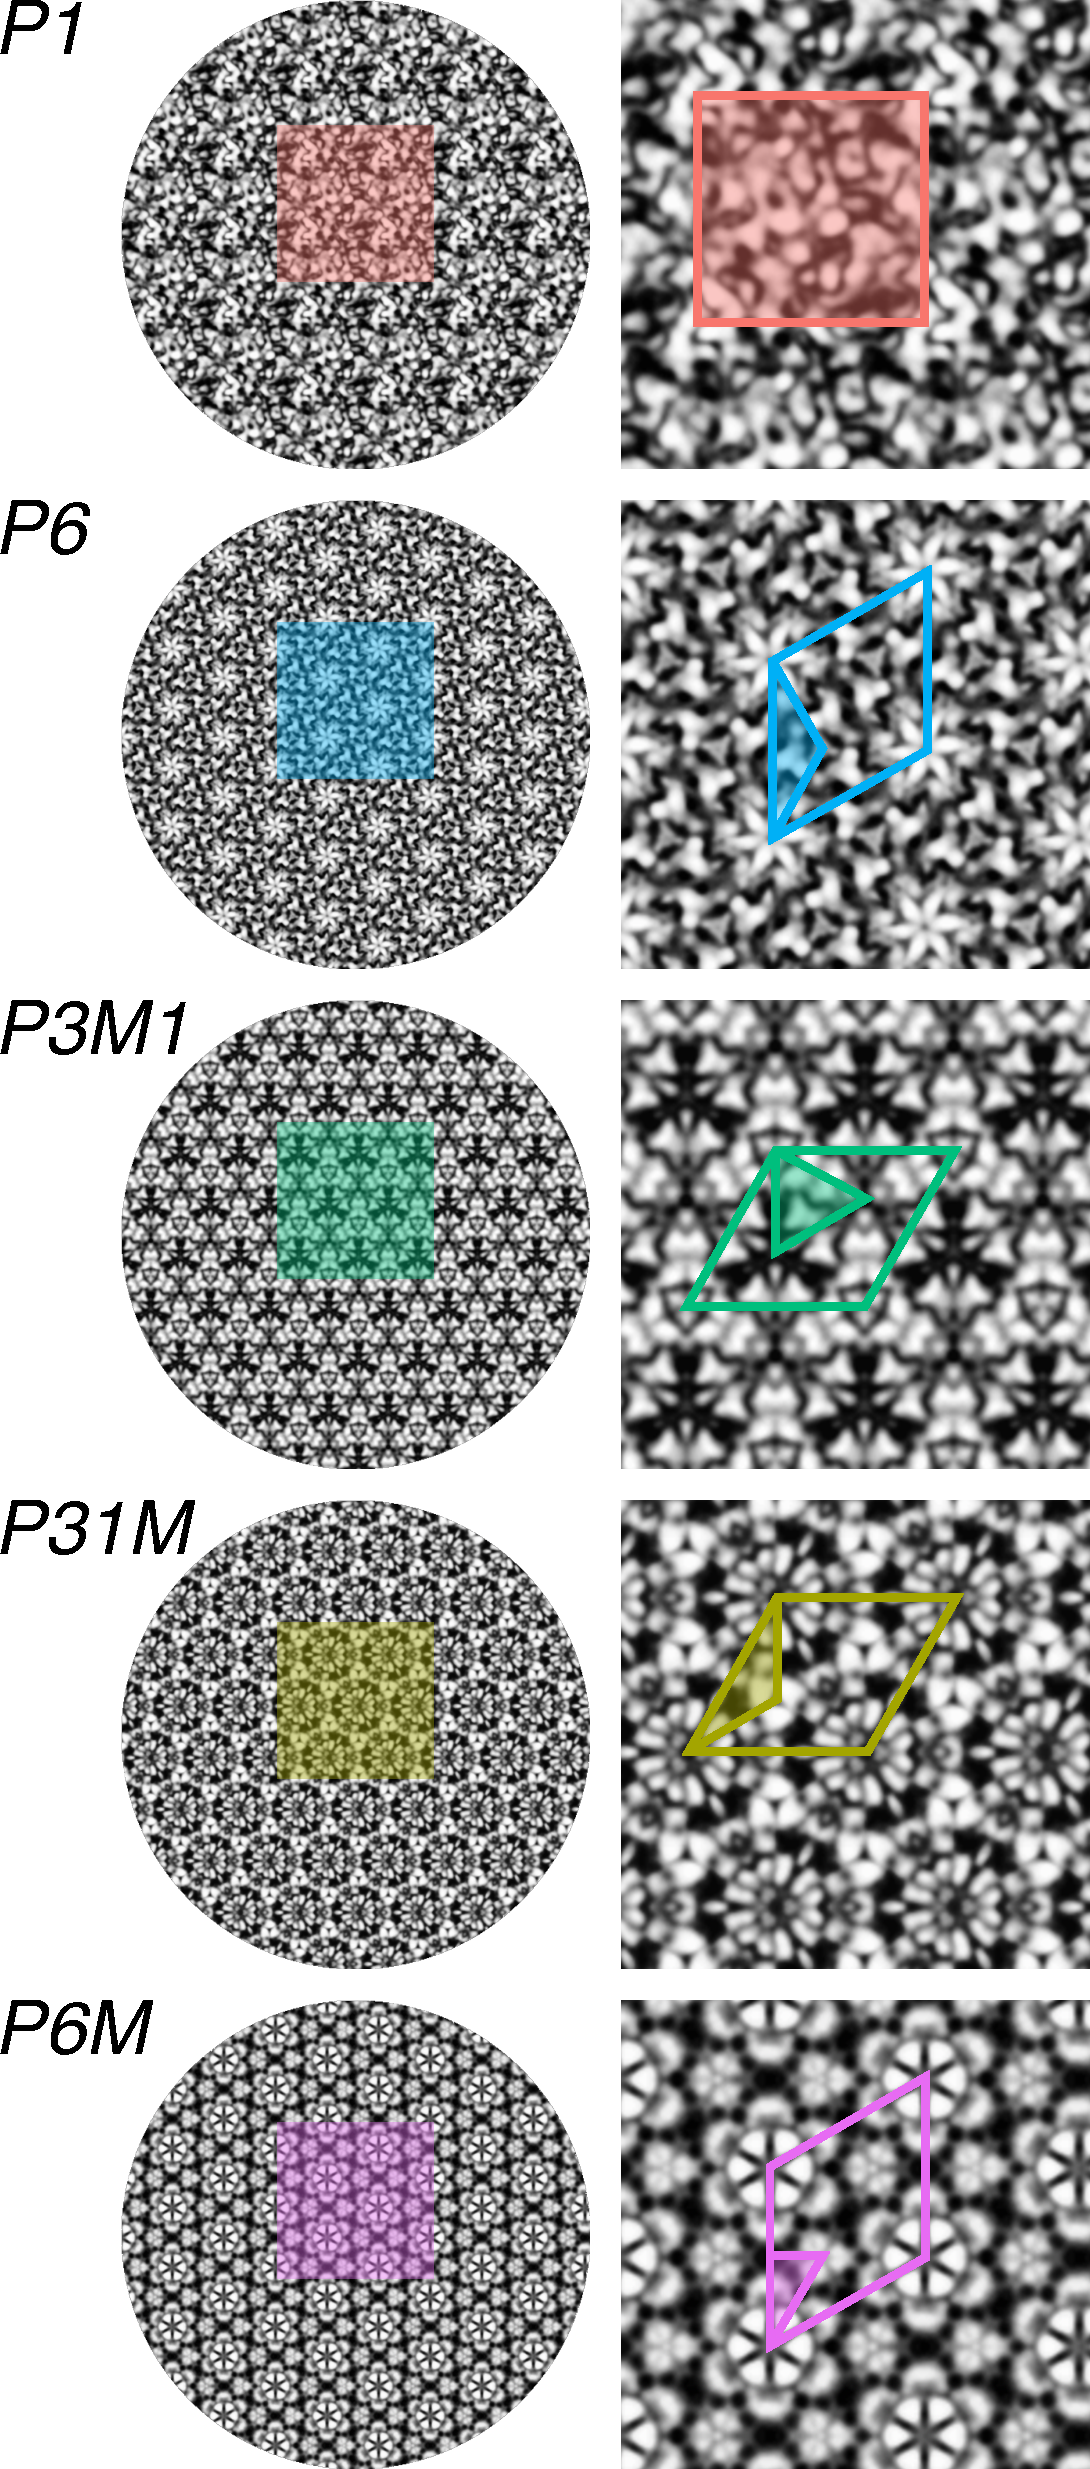
\includegraphics[scale=0.3]{./figures/wpg_structure.pdf}
	\caption{The fundamental region and lattice structure of the five wallpaper groups used in the study. The complete wallpaper is shown in the left-hand column with a shaded region that is repeated and enlarged in the right-hand column. The colored outline in the enlarged region indicates the repeating lattice for each group, while the shaded area indicates the fundamental region (see text). For \textit{P1}, the fundamental region covers the entire lattice. Note that even though \textit{P6} and \textit{P31M} have the same fundamental region and lattice shapes, they differ in terms of the symmetries present within the lattice---most notably, \textit{P31M} contains reflection symmetry, while \textit{P6} does not. The symmetry content of each group is detailed on the wallpaper group wikipedia page (\url{https://en.wikipedia.org/wiki/Wallpaper_group}, accessed on 14/4/2022)}
	\label{fig:wpg_structure}
\end{figure}

Participants were given 20 exemplars, all belonging to same group (see Figure \ref{fig:wpg_exemplars} for a selection of the exemplars, and Section \ref{methods} for details on how they were created) and asked to freely sort them into as many subsets as they wished. Participants sorted exemplars belonging to five different wallpaper groups, one group at a time. This approach allowed us to compare the five wallpaper groups, both in terms of how many subsets participants generated, and also in terms of the \textit{Jaccard index}, a summary statistic capturing the similarity across exemplar pairs for each group. Within each group, we were also able to identify exemplar pairs that were rated as highly similar and highly dissimilar. Our main conclusion is that \textit{P1} was systematically more self-similar than the any other groups, while the other four groups could not be distinguished on these measures. We also demonstrate that for all five groups, participants consistently group certain pairs of exemplars together, although the number of consistent pairs varies among groups. Our results open the door to further investigations into the psychological and neural mechanisms that drive perceptual similarity among wallpaper group exemplars, and indeed among exemplars from different classes of structured patterns. 

\begin{figure}[H]

	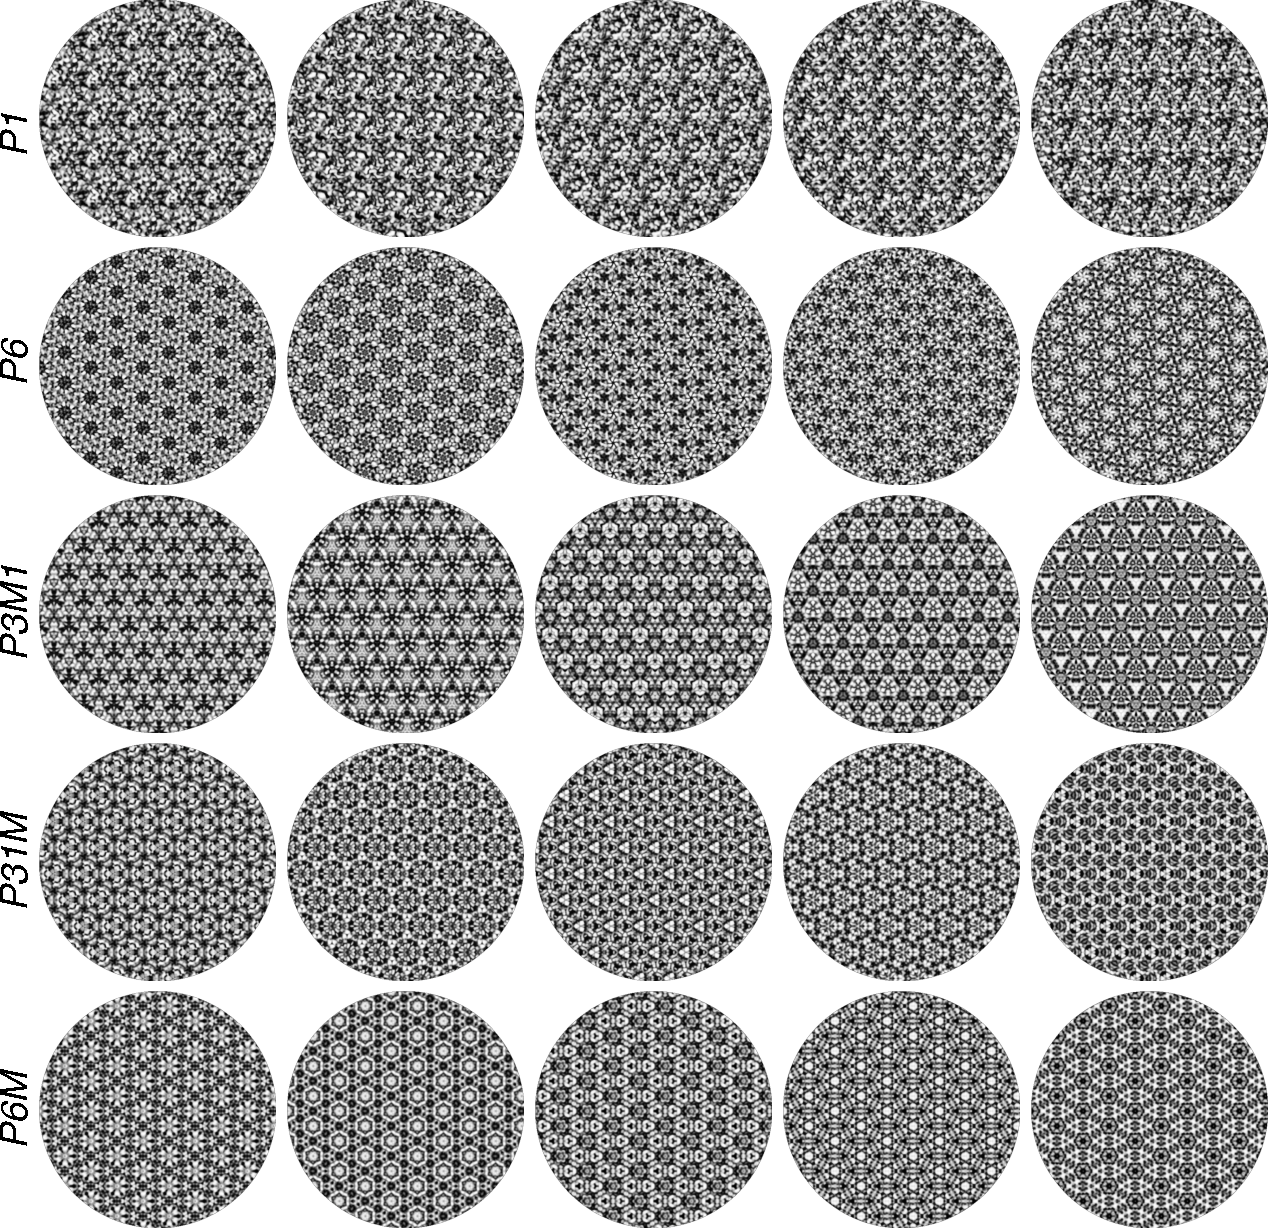
\includegraphics[scale=0.6]{./figures//wpg_exemplars.pdf}
	\caption{Five of the twenty exemplars used for each group are shown to highlight the diversity\linebreak among exemplars.}
	\label{fig:wpg_exemplars}
\end{figure}

\section{Results}
Wallpaper group \textit{P1} was more self-similar than the other four groups. This was evident in the number of sets generated for this group across participants, which was lower for \textit{P1} (median = 3) than for the four other groups (median = 4--5, see Figure \ref{fig:n_sets_jaccard_summary}). We confirmed this observation statistically by running a repeated measures analysis of variance (ANOVA), which revealed a significant effect of group ($F(4, 124) = 7.330, p < 0.0001)$). Post hoc pairwise \textit{t}-tests showed that the mean number of sets was lower for \textit{P1} than all other groups ($ps < 0.005$), but no other means differed (see Table \ref{table:t-stats}).


Next, we computed the Jaccard index (see \ref{methods}) across participants for every pairwise combination of exemplars in each group. This provides a measure of the similarity between exemplars within each group. \textit{P1} had systematically higher Jaccard indices than the four other groups (see \mbox{Figure \ref{fig:n_sets_jaccard_summary}}), as confirmed by a repeated measures ANOVA, which revealed a statistically significant effect of group ($F(4, 495)=20.178, p < 0.0001$). The post hoc \textit{t}-tests showed that \textit{P1} had higher Jaccard indices than all other groups ($ps < 0.0001$; see Table \ref{table:t-stats}). The fact that the group (\textit{P1}) for which fewer subsets were generated also had higher Jaccard indices than the other groups illustrates the inherent link between the two measures. For wallpaper groups where the 20 exemplars are sorted into fewer subsets, each individual exemplar pair is more likely to be a member of the same subset, and less likely to be a member of distinct subsets. This in turn leads to higher Jaccard indices. Our pairwise \textit{t}-tests also showed that \textit{P31M} had lower Jaccard indices than \textit{P6} ($p = 0.037$). This effect does not pass our Bonferroni-corrected threshold for significance ($\alpha < 0.005$, but may nonetheless possibly reflect real differences in how consistently exemplars were grouped together across participants. Shortly, we will explore this idea more in depth. Out of the five groups tested, \textit{P1} is the only one that can be reliably differentiated based on our measures, being higher in self-similarity among the exemplars, and thus lower in diversity among the exemplars. 


\begin{figure}[H]

	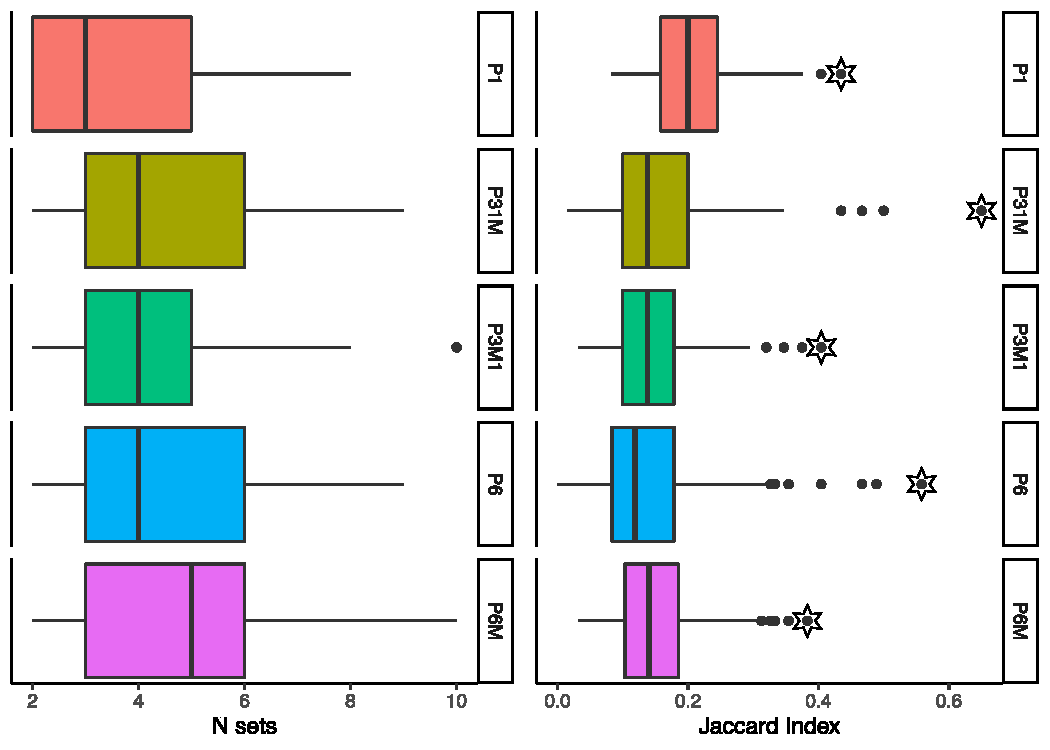
\includegraphics[scale=0.65]{./figures/nsets_jaccard_summary.pdf}
	\caption{Left panel: Boxplots showing the number of subsets generated by participants for each of the wallpaper groups. Right panel: Boxplots showing Jaccard indices for every pairwise combination of exemplars in each of the wallpaper groups. Note that each data point here is the Jaccard index for a particular exemplar pair calculated across participants, unlike the left panel where each data point is a participant. The exemplar pairs with the highest Jaccard indices have been highlighted with stars. Those outlier pairs are explored further in Figure \ref{fig:jaccard_inspection}. For both panels, the lower box boundary is the 25th percentile. The dark line in the box is the median. The upper box boundary is the 75th percentile. The “whiskers” show $-$/+ the interquartile range * 1.5. }
	\label{fig:n_sets_jaccard_summary}
\end{figure}


\vspace{-6pt}
\begin{table}[H]
\caption{Results of post hoc pairwise \textit{t}-tests on number of sets and Jaccard Indices. The degrees of freedom was 945 for the Jaccard Index test. For the number of sets test, the degrees of freedom had to be adjusted to account for the fact that one participant did not report number of sets for P6M (see \ref{methods}), and ranged between 127.0 and 127.1.\label{table:t-stats}}
	\begin{adjustwidth}{-\extralength}{0cm}
		\newcolumntype{C}{>{\centering\arraybackslash}X}
		\begin{tabularx}{\textwidth+\extralength}{CCCCCCC}
			\toprule
	 & \multicolumn{3}{c}{\textbf{Number of Sets}} & \multicolumn{3}{c}{\textbf{Jaccard Index}} \\ \midrule 
	\textbf{Pairs} & \textit{\textbf{t}} & \textit{\textbf{p}} & \textit{\textbf{D}} & \textit{\textbf{t}} & \textit{\textbf{p}} & \textit{\textbf{D}} \\ \midrule
	\textit{P1 vs. P31M} & $-$2.981 & 0.0034 & $-$0.734 & 5.641 & $<$0.0001 & 0.579 \\ \midrule 
	\textit{P1 vs. P3M1} & $-$3.423 & 0.0008 & $-$0.843  & 7.233 & $<$0.0001 & 0.742 \\ \midrule
	\textit{P1 vs. P6} & $-$4.748 & $<$0.0001 & $-$1.169 & 7.734 & $<$0.0001 & 0.794 \\ \midrule
	\textit{P1 vs. P6M} & $-$4.553 & $<$0.0001 & $-$1.132  & 6.946 & $<$0.0001 & 0.713 \\ \midrule
	\textit{P31M vs. P3M1} & $-$0.442 & 0.6595 & $-$0.109 & 1.592 & 0.1117 & 0.163 \\ \midrule
	\textit{P31M vs. P6} & $-$1.767 & 0.0797 & $-$0.435 & 2.094 & 0.0366 & 0.215 \\ \midrule
	\textit{P31M vs. P6M} & $-$1.600 & 0.1120 & $-$0.398 & 1.305 & 0.1921 & 0.134 \\ \midrule
	\textit{P3M1 vs. P6} & $-$1.325 & 0.1875 & $-$0.326 & 0.502 & 0.6160 & 0.051 \\ \midrule
	\textit{P3M1 vs. P6M} & $-$1.163 & 0.2470 & 0.289 & $-$0.287 & 0.7745 & $-$0.029 \\ \midrule
	\textit{P6 vs. P6M} & 0.150 & 0.8814 & 0.037 & -0.788 & 0.4307 & -0.081 \\
			\bottomrule
		\end{tabularx}
	\end{adjustwidth}
	
\end{table}








In order to quantify the extent to which exemplars were consistently grouped together, we ran a permutation analysis in which exemplar labels were shuffled among the sets generated for each participant (see \ref{methods}). This provides, for each group, the expected distribution of Jaccard indices for every pairwise combination of exemplars, if exemplars were assigned randomly to subsets. Moreover, the analysis allows us to compute an empirical \textit{z}-score that expressed the extent to which a given pair of exemplars deviates from the random assignment. 

Because the random distribution is generated by shuffling exemplars across the specific sets generated by each participant for each group, this \textit{z}-score is independent of the number of sets. If for a given group, none of the pairs deviate significantly from the random distribution, it would indicate that no exemplar pairs were consistently grouped together across participants. To estimate the extent to which this is the case, we look at the distribution of \textit{z}-scores across the pairs for each group, as plotted in Figure \ref{fig:jaccard_permutation}, and count the number of pairs for each group for which the \textit{p}-value associated with the threshold exceeds a given $\alpha$ value. At a threshold of $\alpha = 0.01$, several pairs survive for all groups, and even at a much more conservative criterion of $\alpha = 0.0001$, most groups have more than one pairing that survives (see Table \ref{table:pairings}). It is worth noting that the latter threshold ($\alpha = 0.0001$) is lower than the $\alpha$ associated with a Bonferroni correction within the group, given that there are 190 pairs per group: \[ \alpha = \frac{0.05}{190} = 0.0003 \] 

Thus, we conclude that for several exemplar pairs, participants are consistent in how they tend to pair the exemplars. It is interesting to consider that this measure of consistency might provide another way of differentiating wallpaper groups in terms of perceptual self-similarity. While groups \textit{P31M}, \textit{P3M1}, \textit{P6} and \textit{P6M} have comparable Jaccard scores (see Figure \ref{fig:n_sets_jaccard_summary}), they differ in the number of consistent pairings, with \textit{P31M} and \textit{P6} producing more consistent pairs than the other two (see Figure \ref{fig:jaccard_permutation}). 


\begin{table}[H] 
\caption{Number of consistent pairings at two different $\alpha$-levels for the five groups.\label{table:pairings}}
\newcolumntype{C}{>{\centering\arraybackslash}X}
\begin{tabularx}{\textwidth}{CCC}
\toprule
		\multicolumn{3}{c}{\textbf{Consistent Pairings}} \\
		\midrule
		\textbf{Group} & $\boldsymbol{p<0.01}$ & $\boldsymbol{p<0.0001}$ \\
		\midrule
		\textit{P1}   & 6  & 1  \\
		\textit{P31M} & 17 & 10 \\
		\textit{P3M1} & 12 & 3  \\
		\textit{P6}   & 17 & 11 \\
		\textit{P6M}  & 15 & 4  \\
\bottomrule
\end{tabularx}
\end{table}




The Jaccard indices also allow us to focus on exemplar pairs that have a high level of similarity relative to the rest of the pairs in the set. We do this by identifying outlier pairs from each group in terms of Jaccard indices, as identified with stars in Figure \ref{fig:n_sets_jaccard_summary}. Because the Jaccard indices are computed across participants, these outliers are also among the pairs most consistently sorted together, as identified in Figure \ref{fig:jaccard_permutation}. For each exemplar in each outlier pair, we can visualize the pairwise similarity (as measured by the Jaccard index) to every other exemplar in the set (see \ref{fig:jaccard_inspection}). That is, we can visualize portions of the network of perceived similarity within a set of exemplars. Future work could probe the extent to which networks of perceived similarity have similar structure across wallpaper groups and examine what perceptual features best account for participants' perceptions of exemplar similarity.

\begin{figure}[H]
	
	\includegraphics[width=.9\linewidth]{./figures/jaccard_inspection.pdf}
	\caption{For each wallpaper group, we identified the two most self-similar exemplars, the same pair that is indicated by the right-most datapoint for each group in Figure \ref{fig:jaccard_permutation}. The two circular network plots are showing the pairwise similarities between those two exemplars and every other exemplar in the set. The pairwise similarities across all exemplars are plotted as a similarity matrix and on the rightmost side of the plot, the two most self-similar exemplars (bottom) are plotted with the exemplar that was least similar to both (top). The connecting lines between the exemplars indicate the similarity.}
	\label{fig:jaccard_inspection}
\end{figure}



\begin{figure}[H]
	
	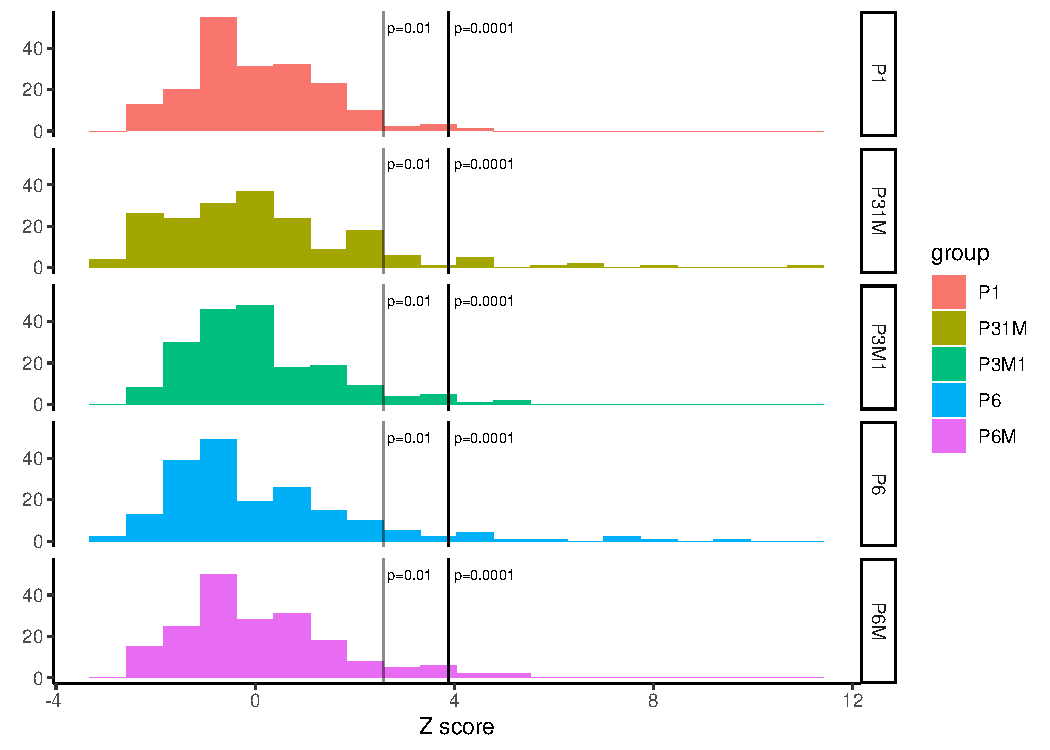
\includegraphics[width=.85\linewidth]{./figures/emp-jaccard-histogram-w-annotations-no-hyphen.pdf}
	\caption{Distribution of \textit{z}-scores across the 190 pairs in each of the five wallpaper groups. The two lines indicate the \textit{z}-scores associated with $\alpha$ of 0.01 and 0.0001, respectively.}%mdpi: Please change the hyphen(-) into minus sign(−).
	\label{fig:jaccard_permutation}
\end{figure}
\section{Discussion}
Previous work has demonstrated that the visual cortex of both humans and macaque monkeys carries highly detailed representations of the symmetries within wallpaper groups, as evidenced by systematic differences in the magnitude of the response elicited by different groups \citep{RN1725,RN1959,kohler_clarke_2021,audurier_symmetry_2021}. This distinction between groups can also be observed in psychophysical threshold measurements \citep{kohler_clarke_2021}, although observers may not have a strong awareness of the wallpaper group membership of individual exemplars \citep{RN172}. In the current study, we explored a new piece of the story about how wallpaper groups are processed by the visual system, namely the issue of how self-similar different exemplars from the \textit{same} wallpaper group appear to untrained observers. We tested this by asking participants to spontaneously sort 20 exemplars from each of five wallpaper groups into different subsets. 

Our first finding concerns the number of subsets generated for each group. We find that \textit{P1} is divided into fewer subsets than the other four groups. This indicates that the limited complexity of this group, which contains only translation symmetry, has a direct effect of the number of distinct subsets. The relationship between complexity/symmetry content and number of subsets produced is not straightforward, however, as indicated by the fact that \textit{P6M} is not consistently grouped into more subsets than \textit{P6}, \textit{P3M1} and \textit{P31M}, despite the fact that these other groups all contain fewer symmetries than \textit{P6M}. We speculate that this lack of further differentiation is a result of an upper limit on how additional complexity can influence perceptual self-similarity. However, future work with additional wallpaper groups, including groups that are relatively low in complexity but high in %Please verify.
 self-similarity (e.g., \textit{P2} and \textit{PMM}, see \citep{RN172}), is needed to draw firm conclusions about this hypothesis.

It is important to note that \textit{P6}, \textit{P3M1} and \textit{P31M} all consistently generate weaker brain activity than \textit{P6M}, and produce higher thresholds in a symmetry detection task \citep{kohler_clarke_2021}. Our results would therefore suggest that there is no clear relationship between the strength of the visual system's response to symmetries in the wallpaper group, and the perceptual self-similarity of each individual group. Future work should explore this more closely, and look for neural correlates of similarity among exemplars from the same group.

We also computed Jaccard indices that, for every possible exemplar pair, expresses the frequency of those two exemplars being grouped together. As described above, the average Jaccard index for a group is inherently linked to the number of subsets produced for that group, because fewer subsets mean that exemplars are more likely to be made members of the same pair, and less likely to be made members of the same pair. It is therefore not surprising that we find the same general pattern for Jaccard indices and the number of subsets, namely that \textit{P1} has higher indices than the other groups. The advantage of the Jaccard indices, however, is that they allow us to conduct a permutation analysis that quantifies the extent to which pairs of exemplars are consistently grouped together across participants, independent of the number of sets produced for a given group. It is important to note that consistency in the choice of which exemplars to group into subsets is not an unavoidable consequence of our experimental design, and it does not follow naturally from the results described so far. It would be perfectly possible for participants to group the sets together, producing fewer subsets for \textit{P1} as observed, but exhibit no consistency across participants at all. That is not what we see, however. Even when setting a conservative threshold, all five groups produce one or more pairs that are consistently grouped together, demonstrating that the sorting of exemplars into subsets is not done randomly or arbitrarily across the participants. Rather, different individuals agree to some extent on which exemplars belong together. Because our measure of consistency is independent of the number of subsets produced for a given group, it allows us to show that although \textit{P1} has the highest overall Jaccard indices (as a result of the fewer sets produced for this group), it in fact produces fewer consistent pairs than other groups (see Table \ref{table:pairings}). Indeed, the participants made few comments about their own sorting strategies, but most observed that P1 exemplars were the most difficult to sort because of the lack of readily apparent features that were consistent across exemplars.

In sum, we find consistencies in the way that untrained human observers sort wallpaper images. Observers sort exemplars with translational symmmetry alone (\textit{P1}) into smaller numbers of sets than exemplars with rotation or reflection symmetry. On average, pairs of \textit{P1} exemplars are sorted together more often than exemplars from other wallpaper groups. At the same time, some specific exemplar pairs from wallpaper groups with 3- or 6- fold rotational or reflection symmetry are sorted together substantially more often than predicted by chance.

We note that that the spontaneous sorting task our observers engaged in has less intrinsic structure than some other tasks used to study similar questions such as oddball detection \citep{RN1253,Hebart2020-so,Landwehr2011-kg}, and thus may involve somewhat different perceptual and cognitive processes. In particular, wallpaper group exemplars have a reduced dimensionality relative to natural objects. Even so, large scale evaluations of how human observers perceive similarity in natural objects yield dimensions that appear to relate to the strict regularities observed in wallpapers: round shape, patterning and repetition \citep{Hebart2020-so}. In future work, it would be interesting to explore whether different behavioral tasks yield comparable similarity spaces, or more generally, how task demands shape similarity judgments.

In conclusion, our results suggest that human observers show sensitivity to the dimensions of 2D symmetry (translation, rotation and reflection) embedded in wallpaper exemplars. However, their sorting behavior demonstrates only weak evidence that group-theoretic measures of symmetry influence the perception of self-similarity. These results contribute to a small, but growing literature on the perception of visual aesthetics \citep{Carneiro2012-ph,Graham2010-yf,Friedenberg2012-gf,Laine-Hernandez2008-sg,Richards1972-gl}, where symmetry is one of many contributing factors.

\section{Materials and Methods}
\label{methods}

\subsection{Participants}
A total of 33 participants (9 Male, 24 Female), ranging in age between 18 and 35 completed this study. The participants were recruited from the undergraduate participant pool in the Department of Psychology at the The Pennsylvania State University. All participants had self- reported 20/20 or corrected to 20/20 vision. We obtained written informed consent to participate from all participants under procedures approved by the Institutional Review Board of The Pennsylvania State University (\#38536). The research was conducted according to the principles expressed in the Declaration of Helsinki. Participants include \textit{n}=11 collected and described in \citep{vedak_thesis}, plus an additional group collected at a later date using the same protocol.

\subsection{Stimulus Generation}
Five wallpaper groups (\textit{P1}, \textit{P6}, \textit{P3M1}, \textit{P31M} and \textit{P6M}) were selected for use in the study. The selection was motivated partially by the fact that all five groups has previously been demonstrated to be high in self-similarity \citep{RN172}, and partially by the fact that \textit{P3M1}, \textit{P31M}, \textit{P6} and \textit{P6M} all share the same lattice shape. We also found it interesting that while \textit{P6}, \textit{P3M1} and \textit{P31M} differ in their symmetry content, all are subgroups of \textit{P6M} with index 2, which means that \textit{P6M} can be generated by adding one additional transformation to \textit{P6}, \textit{P3M1} or \textit{P31M} \citep{kohler_clarke_2021}. A total of 20 exemplars from each of these five wallpaper groups were generated using a modified version of the methodology developed by Clarke and colleagues \citep{RN172} that we have described in detail elsewhere \citep{RN1725}. Briefly, exemplars belonging to each group were generated by starting with a random-noise patch, which was then repeated and transformed to tile the image plane, in accordance with the symmetry axes and geometric lattice specific to each group. The use of noise patches as the starting point for stimulus generation makes it possible to create an almost unlimited number of distinct exemplars from each wallpaper group. To make individual exemplars as similar as possible we replaced the power spectrum of each exemplar with the median across exemplars within a group. These images were printed onto white cardstock and cut into squares, allowing participants to manipulate the orientation of the images during the sorting tasks. Five exemplars from each group are shown (in reduced size) in Figure \ref{fig:wpg_exemplars}. 

\subsection{Procedure}
Participants were presented with the 20 exemplars of a single wallpaper group (i.e., \emph{P1}, \emph{P3M1}, \emph{P31M}, \emph{P6}, \emph{P6M}) and instructed to sort them into subsets by placing them into piles. Participants were advised to sort the exemplars into as many piles as they deemed necessary based on whatever criteria they desired. There were no time constraints placed on this sorting task, and the participants were allowed to move exemplars between piles until they were satisfied with their classification. This method was then repeated for the remaining four wallpaper groups for each participant, with group presentation order randomized between participants. These tasks were carried out on a large table with sufficient space to randomly lay out all twenty exemplars of each set, illuminated by normal overhead room lighting. Upon completion of each sorting task, participants were asked to verbalize which features they used to sort the exemplars. After completion of all five sorting tasks, participants were asked whether they had a distinct method for sorting the images, and whether any wallpaper group was particularly easy or difficult to sort.

\subsection{Generating the Jaccard Index}
The data were prepared for analysis by creating one binary variable for each subset created by each participant within a sorting task. Then, each exemplar was assigned a value of one (1) if it was included in a subset, or a value zero (0) if it was not. Next, the similarity of each pair of exemplars within a sorting task was calculated using the Jaccard index, as a measure of similarity and diversity for the binary data. This index is calculated by \mbox{the equation}  \[ J = \frac{x}{x + y + z} \] with \emph{x} representing the number of subsets that contained both exemplars, and \emph{y} and \emph{z} the number of subsets that contain only one exemplar of the pair \citep{capra_factor_2005}, across participants. Thus, the Jaccard index is the ratio of the number of subsets containing both exemplars of a pair to the number of subsets containing at least one of the exemplars of a pair, thereby excluding subsets with joint absences.

\subsection{Statistical Analysis}
We tested for differences between the five wallpaper groups tested in terms of number of sets produced and Jaccard indices by running repeated measures analyses of variance (rmANOVA) with group as a fixed factor and participant as a random factor. We then tested the extent to which differences between specific pairs of wallpaper groups contributed to any rmANOVA effects found, by running post hoc paired \textit{t}-tests comparing every possible pairing of the wallpaper groups, for both number of sets and Jaccard Indices. Because there were 10 possible pairings of the groups, we applied the Bonferroni-correction and adjusted our $\alpha$-level so that each \textit{t}-test was only considered significant if $p < 0.005$. The number of datasets was missng for one participant for the wallpaper group \textit{P6M}; thus, the degrees of freedom used in the paired \textit{t}-tests was adjusted using the Kenward--Roger technique---the default in the \textit{emmeans} package in R.

We ran a permutation analysis in order to quantify the extent to which pairs of exemplars were consistently grouped together, across participants. This involved generating a randomized dataset, as follows. For each participant and wallpaper group, we randomized which specific exemplars were sorted together. This retained the basic structure of each participants' sorting data---the number of subsets created---but randomized the relationship between specific wallpaper exemplars that were sorted together across the participants. We then created 1000 such permuted datasets, and calculated the Jaccard index for each exemplar pair within each group for each of the permuted datasets. This permitted the calculation of an \emph{empirical} Jaccard index based on the permuted data from which distributional statistics such as \textit{z} could be calculated. The \emph{observed} Jaccard indices for each exemplar pair were then compared to the empirically-derived reference distribution to determine which exemplar pairs were sorted together more frequently than chance would predict.



\vspace{6pt} 

%%%%%%%%%%%%%%%%%%%%%%%%%%%%%%%%%%%%%%%%%%
%% optional
%\supplementary{The following are available online at \linksupplementary{s1}, Figure S1: title, Table S1: title, Video S1: title.}

% Only for the journal Methods and Protocols:
% If you wish to submit a video article, please do so with any other supplementary material.
% \supplementary{The following are available at \linksupplementary{s1}, Figure S1: title, Table S1: title, Video S1: title. A supporting video article is available at doi: link.} 

%%%%%%%%%%%%%%%%%%%%%%%%%%%%%%%%%%%%%%%%%%
\authorcontributions{Conceptualization, R.O.G. and S.V.; methodology, R.O.G. and S.V.; data collection, S.V.; data analysis, P.J.K. and R.O.G.; data curation, R.O.G.; writing---original draft preparation, P.J.K., S.V. and R.O.G.; writing---review and editing, P.J.K. and R.O.G.; visualization, P.J.K. and R.O.G.; funding acquisition, P.J.K. and R.O.G.}

\funding{This work was supported by National Science Foundation INSPIRE grant IIS-1248076 awarded to Yanxi Liu, Anthony M. Norcia and R.O.G., by the Vision Science to Applications (VISTA) program funded by the Canada First Research Excellence Fund (CFREF, 2016–2023) and by a Discovery Grant from the Natural Sciences and Engineering
429 Research Council of Canada awarded to P.J.K.}

\institutionalreview{The study was conducted according to the guidelines of the Declaration of Helsinki, and approved by the Institutional Review Board of The Pennsylvania State University (\#38536).}

\informedconsent{Informed consent was obtained from all subjects involved in the study.}

\dataavailability{Data and code required to reproduce analyses and results figures can be found in the following github repository: \url{https://github.com/gilmore-lab/symmetry-sorting}}

\acknowledgments{We thank two reviewers for comments which helped improve the paper.}

\conflictsofinterest{The authors declare no conflict of interest.} %Declare conflicts of interest or state ``The authors declare no conflict of interest.'' Authors must identify and declare any personal circumstances or interest that may be perceived as inappropriately influencing the representation or interpretation of reported research results. Any role of the funders in the design of the study; in the collection, analyses or interpretation of data; in the writing of the manuscript, or in the decision to publish the results must be declared in this section. If there is no role, please state ``The funders had no role in the design of the study; in the collection, analyses, or interpretation of data; in the writing of the manuscript, or in the decision to publish the~results''.
% Bibliography

\begin{adjustwidth}{-\extralength}{0cm}

\reftitle{References}
\begin{thebibliography}{999}

\bibitem[Liu \em{et~al.}(2010)Liu, Hel-Or, Kaplan, and Van~Gool]{RN1425}
Liu, Y.; Hel-Or, H.; Kaplan, C.S.; Van~Gool, L.
\newblock Computational Symmetry in Computer Vision and Computer Graphics.
\newblock {\em Found. Trends Comput. Graph. Vis.} {\bf
  2010}, {\em 5},~1--195.
\newblock
  doi:{\changeurlcolor{black}\href{https://doi.org/10.1561/0600000008}{\detokenize{10.1561/0600000008}}}.

\bibitem[Fedorov(1891)]{RN1562}
Fedorov, E.
\newblock Symmetry in the plane.
\newblock  Zapiski Imperatorskogo S. Peterburgskogo Mineralogichesgo
  Obshchestva. \emph{Proc. S. Peterb. Mineral. Soc.}  \textbf{1891}, \emph{2},  345--390.

\bibitem[Polya(1924)]{RN1563}
Polya, G.
\newblock XII. Über die Analogie der Kristallsymmetrie in der Ebene.
\newblock {\em Z. FüR Krist. Cryst. Mater.} {\bf
  1924}, {\em 60},~278--282.

\bibitem[Mach(1959)]{mach_1959}
Mach, E.
\newblock \emph{The {Analysis} of {Sensations} (1897)};
\newblock   Dover: New York, NY, USA,  1959.

\bibitem[Kohler \em{et~al.}(2016)Kohler, Clarke, Yakovleva, Liu, and
  Norcia]{RN1725}
Kohler, P.J.; Clarke, A.; Yakovleva, A.; Liu, Y.; Norcia, A.M.
\newblock Representation of Maximally Regular Textures in Human Visual Cortex.
\newblock {\em  J. Neurosci.} {\bf 2016}, {\em 36},~714--729.
\newblock
  doi:{\changeurlcolor{black}\href{https://doi.org/10.1523/jneurosci.2962-15.2016}{\detokenize{10.1523/jneurosci.2962-15.2016}}}.

\bibitem[Kohler \em{et~al.}(2018)Kohler, Cottereau, and Norcia]{RN1959}
Kohler, P.J.; Cottereau, B.R.; Norcia, A.M.
\newblock Dynamics of perceptual decisions about symmetry in visual cortex.
\newblock {\em NeuroImage} {\bf 2018}, {\em 167},~316--330.


\bibitem[Kohler and Clarke(2021)]{kohler_clarke_2021}
Kohler, P.J.; Clarke, A.D.F.
\newblock The human visual system preserves the hierarchy of two-dimensional
  pattern regularity.
\newblock {\em Proc. R. Soc. B Biol. Sci.} {\bf
  2021}, {\em 288},~20211142.


\bibitem[Audurier \em{et~al.}(2021)Audurier, Héjja-Brichard, De~Castro,
  Kohler, Norcia, Durand, and Cottereau]{audurier_symmetry_2021}
Audurier, P.; Héjja-Brichard, Y.; De~Castro, V.; Kohler, P.J.; Norcia, A.M.;
  Durand, J.B.; Cottereau, B.R.
\newblock Symmetry {Processing} in the {Macaque} {Visual} {Cortex}.
\newblock {\em Cereb. Cortex} {\bf \hl{2021(Please Add volunme and pages)}}.%MDPI: please add volunme and pages
\newblock
  doi:{\changeurlcolor{black}\href{https://doi.org/10.1093/cercor/bhab358}{\detokenize{10.1093/cercor/bhab358}}}.

\bibitem[Landwehr(2009)]{RN1253}
Landwehr, K.
\newblock Camouflaged symmetry.
\newblock {\em Perception} {\bf 2009}, {\em 38},~1712--1720.

\bibitem[Clarke \em{et~al.}(2011)Clarke, Green, Halley, and Chantler]{RN172}
Clarke, A.D.F.; Green, P.R.; Halley, F.; Chantler, M.J.
\newblock Similar Symmetries: The Role of Wallpaper Groups in Perceptual
  Texture Similarity.
\newblock {\em Symmetry} {\bf 2011}, {\em 3},~246--264.
\newblock
  doi:{\changeurlcolor{black}\href{https://doi.org/10.3390/sym3020246}{\detokenize{10.3390/sym3020246}}}.

\bibitem[Milton \em{et~al.}(2008)Milton, Longmore, and Wills]{Milton2008-ez}
Milton, F.; Longmore, C.A.; Wills, A.J.
\newblock Processes of overall similarity sorting in free classification.
\newblock {\em J. Exp. Psychol. Hum. Percept. Perform.} {\bf 2008}, {\em 34},~676--692.
\newblock
  doi:{\changeurlcolor{black}\href{https://doi.org/10.1037/0096-1523.34.3.676}{\detokenize{10.1037/0096-1523.34.3.676}}}.

\bibitem[Pothos \em{et~al.}(2011)Pothos, Perlman, Bailey, Kurtz, Edwards,
  Hines, and McDonnell]{Pothos2011-vi}
Pothos, E.M.; Perlman, A.; Bailey, T.M.; Kurtz, K.; Edwards, D.J.; Hines, P.;
  McDonnell, J.V.
\newblock Measuring category intuitiveness in unconstrained categorization
  tasks.
\newblock {\em Cognition} {\bf 2011}, {\em 121},~83--100.
\newblock
  doi:{\changeurlcolor{black}\href{https://doi.org/10.1016/j.cognition.2011.06.002}{\detokenize{10.1016/j.cognition.2011.06.002}}}.

\bibitem[Hebart \em{et~al.}(2020)Hebart, Zheng, Pereira, and
  Baker]{Hebart2020-so}
Hebart, M.N.; Zheng, C.Y.; Pereira, F.; Baker, C.I.
\newblock Revealing the multidimensional mental representations of natural
  objects underlying human similarity judgements.
\newblock {\em Nat. Hum. Behav.} {\bf 2020}, {\em 4},~1173--1185.
\newblock
  doi:{\changeurlcolor{black}\href{https://doi.org/10.1038/s41562-020-00951-3}{\detokenize{10.1038/s41562-020-00951-3}}}.

\bibitem[Landwehr(2011)]{Landwehr2011-kg}
Landwehr, K.
\newblock Visual Discrimination of the 17 Plane Symmetry Groups.
\newblock {\em Symmetry} {\bf 2011}, {\em 3},~207--219.
\newblock
  doi:{\changeurlcolor{black}\href{https://doi.org/10.3390/sym3020207}{\detokenize{10.3390/sym3020207}}}.

\bibitem[Carneiro \em{et~al.}(2012)Carneiro, da~Silva, Del~Bue, and
  Costeira]{Carneiro2012-ph}
Carneiro, G.; da~Silva, N.P.; Del~Bue, A.; Costeira, J.P.
\newblock Artistic Image Classification: An Analysis on the {PRINTART}
  Database.
\newblock  In \emph{Computer Vision--{ECCV} 2012}; Springer: Berlin/Heidelberg,  Germany, 2012;  pp. 143--157.
\newblock
  doi:{\changeurlcolor{black}\href{https://doi.org/10.1007/978-3-642-33765-9\_11}{\detokenize{10.1007/978-3-642-33765-9\_11}}}.

\bibitem[Graham \em{et~al.}(2010)Graham, Friedenberg, Rockmore, and
  Field]{Graham2010-yf}
Graham, D.J.; Friedenberg, J.D.; Rockmore, D.N.; Field, D.J.
\newblock Mapping the similarity space of paintings: Image statistics and
  visual perception.
\newblock {\em Vis. Cogn.} {\bf 2010}, {\em 18},~559--573.
\newblock
  doi:{\changeurlcolor{black}\href{https://doi.org/10.1080/13506280902934454}{\detokenize{10.1080/13506280902934454}}}.

\bibitem[Friedenberg(2012)]{Friedenberg2012-gf}
Friedenberg, J.
\newblock Aesthetic judgment of triangular shape: compactness and not the
  golden ratio determines perceived attractiveness.
\newblock {\em i-Perception} {\bf 2012}, {\em 3},~163--175.
\newblock
  doi:{\changeurlcolor{black}\href{https://doi.org/10.1068/i0484}{\detokenize{10.1068/i0484}}}.

\bibitem[Laine-Hernandez and Westman(2008)]{Laine-Hernandez2008-sg}
Laine-Hernandez, M.; Westman, S.
\newblock Multifaceted image similarity criteria as revealed by sorting tasks.
\newblock {\em Proc. Am. Soc. Inf. Sci. Technol.} {\bf 2008}, {\em 45},~1--14.
\newblock
  doi:{\changeurlcolor{black}\href{https://doi.org/10.1002/meet.2008.1450450256}{\detokenize{10.1002/meet.2008.1450450256}}}.

\bibitem[Richards(1972)]{Richards1972-gl}
Richards, L.G.
\newblock A multidimensional scaling analysis of judged similarity of complex
  forms from two task situations.
\newblock {\em Percept. Psychophys.} {\bf 1972}, {\em 12},~154--160.
\newblock
  doi:{\changeurlcolor{black}\href{https://doi.org/10.3758/BF03212862}{\detokenize{10.3758/BF03212862}}}.

\bibitem[Vedak(2014)]{vedak_thesis}
Vedak, S.
\newblock The Salience of Lower-Order Features in Highly Self-Similar Wallpaper
  Groups.
\newblock  Honors Thesis, The Pennsylvania State University, State College, PA, 16801, USA, 2014.

\bibitem[Capra(2005)]{capra_factor_2005}
Capra, M.G.
\newblock Factor {Analysis} of {Card} {Sort} {Data}: {An} {Alternative} to
  {Hierarchical} {Cluster} {Analysis}.
\newblock {\em Proc. Hum. Factors Ergon. Soc. Annu. Meet.} {\bf 2005}, {\em 49},~691--695.
  doi:{\changeurlcolor{black}\href{https://doi.org/10.1177/154193120504900512}{\detokenize{10.1177/154193120504900512}}}.

\end{thebibliography}



% Funding
% This work was supported by the Vision Science to Applications (VISTA) program funded by the Canada First Research Excellence Fund (CFREF, 2016–2023) and by a Discovery Grant from the Natural Sciences and Engineering Research Council of Canada awarded to P.J.K. The work was also partially supported by a National Science Foundation INSPIRE grant 1248076 awarded to Yanxi Liu, Anthony M. Norcia and Rick O. Gilmore.
\end{adjustwidth}
\end{document}